\section{From Sets to Groupoids}
\label{sec:groupoids}

From a denotational perspective, a $\Pi$ type $\tau$ denotes a finite set and a
$\Pi$ 1-combinator denotes a permutation on finite sets. This semantics can be
generalized by enriching $\Pi$ types so that they denote more general groupoids
and correspondingly enriching 1-combinators so that they denote
``information-preserving'' transformations on groupoids. The generalization
depends on one crucial insight which is the subject of this section. Briefly
speaking, 1-combinators, their properties, and their operational behavior are
themselves data that can be manipulated by other programs. Depending on the
precise setup, we can use a 1-combinator~$p$ to build one of several kinds of
non-trivial groupoids: an action groupoid $\ag{\tau}{p}$, an iteration groupoid
$\order{p}$, or an inverse order groupoid $\iorder{p}$. We explain these
constructions and then generalize them to a division groupoid $\divg{p}{q}$.

%%%%%
\subsection{$\Pi$ Types as Sets (Discrete Groupoids)}

Each $\Pi$ type $\tau$ denotes a finite set $\sem{\tau}$ as follows:

\[\begin{array}{rcl}
\sem{\zt} &=& \bot \\
\sem{\ot} &=& \top \\
\sem{\tau_1 \oplus \tau_2} &=& \sem{\tau_1} \uplus \sem{\tau_2} \\
\sem{\tau_1 \otimes \tau_2} &=& \sem{\tau_1} \times \sem{\tau_2}
\end{array}\]

\noindent where we use $\bot$ to denote the empty set, $\top$ to denote a set
with one element, and $\uplus$ and~$\times$ to denote the disjoint union of sets
and the cartesian product of sets respectively. Each set can be viewed as a
groupoid whose objects are the set elements and with only identity morphisms on
each object. By only being able to express types whose denotations are trivial
groupoids, $\Pi$ leaves untapped an enormous amount of combinatorial structure
that is expressible in type theory. We show that with a small but deep technical
insight it is possible to extend~$\Pi$ with types whose denotations are
non-trivial ``fractional'' groupoids.

%%%%%
\subsection{Groupoids and Groupoid Cardinality}

There are many definitions of groupoids that provide complimentary perspectives
and insights. Perhaps the simplest definition is that a groupoid is a category
in which every morphism has an inverse. Such a category generally consists of
clusters of connected objects. Each cluster is equivalent (in the
category-theoretic sense) to a group. Thus an alternative definition of a
groupoid is as a generalization of a group that allows for individual elements
to have ``internal symmetries''~\cite{groupoidintro}. Baez et
al.~\cite{2009arXiv0908.4305B} associate with each groupoid a cardinality that
counts the elements up to these ``internal symmetries.''

\begin{definition}[Groupoid Cardinality~\cite{2009arXiv0908.4305B}]
  The cardinality of a groupoid $G$ is the real number:
  \[
    |G| = \sum_{[x]} \frac{1}{|\textsf{Aut}(x)|}
  \]
  provided the sum converges. The summation is over \emph{isomorphism
    classes $[x]$ of objects $x$} and $|\textsf{Aut}(x)|$ is the
  number of {\emph distinct} automorphisms of $x$.
\end{definition}

\begin{figure}[t]
\begin{center}
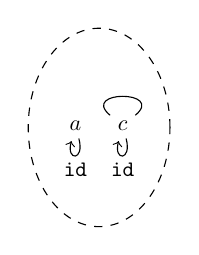
\begin{tikzpicture}[scale=0.6,every node/.style={scale=0.8}]
  \draw[dashed] (0,-0.3) ellipse (1.5cm and 2.1cm);
  \node[below] (A) at (-0.5,0) {$a$};
  \node[below] (C) at (0.5,0) {$c$};
  \path (A) edge [loop below] node[below] {\texttt{id}} (A);
  \path (C) edge [loop below] node[below] {\texttt{id}} (C);
  \path (C) edge [out=140, in=40, looseness=4] (C);
\end{tikzpicture}
\qquad \qquad \qquad
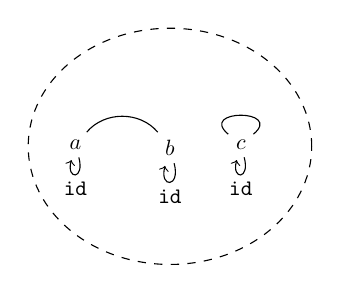
\begin{tikzpicture}[scale=0.6,every node/.style={scale=0.8}]
  \draw[dashed] (0,-0.3) ellipse (3cm and 2.5cm);
  \node[below] (A) at (-2,0) {$a$};
  \node[below] (B) at (0,0) {$b$};
  \node[below] (C) at (1.5,0) {$c$};
  \path (A) edge [bend left=50] (B);
  \path (C) edge [out=140, in=40, looseness=4] (C);
  \path (A) edge [loop below] node[below] {\texttt{id}} (A);
  \path (B) edge [loop below] node[below] {\texttt{id}} (B);
  \path (C) edge [loop below] node[below] {\texttt{id}} (C);
\end{tikzpicture}
\qquad \qquad \qquad
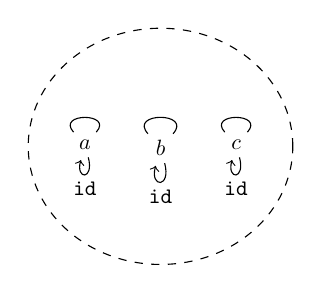
\begin{tikzpicture}[scale=0.6,every node/.style={scale=0.8}]
  \draw[dashed] (0,-0.3) ellipse (2.8cm and 2.5cm);
  \node[below] (A) at (-1.6,0) {$a$};
  \node[below] (B) at (0,0) {$b$};
  \node[below] (C) at (1.6,0) {$c$};
  \path (A) edge [loop below] node[below] {\texttt{id}} (A);
  \path (B) edge [loop below] node[below] {\texttt{id}} (B);
  \path (C) edge [loop below] node[below] {\texttt{id}} (C);
  \path (A) edge [loop above, looseness=3, in=48, out=132] (A);
  \path (B) edge [loop above, looseness=3, in=48, out=132] (B);
  \path (C) edge [loop above, looseness=3, in=48, out=132] (C);
\end{tikzpicture}
\end{center}
\caption{\label{fig:groupoids2}Example groupoids $G_1$, $G_2$, and $G_3$.}
\end{figure}

For plain sets, the definition just counts the elements as each
element is its own equivalence class and has exactly one automorphism
(the identity). For the groupoids $G_1$, $G_2$, and $G_3$ in
Fig.~\ref{fig:groupoids2}, the cardinality of each groupoid is
$\frac{3}{2}$ but for a different reason. Groupoid~$G_1$ consists of
two isomorphism classes: class~$a$ has one object with one
automorphism (the identity) and class~$c$ has one object with two
distinct automorphisms; the cardinality is
$\frac{1}{1} + \frac{1}{2} = \frac{3}{2}$. For groupoid $G_2$, we also
have two isomorphism classes with representatives $a$ and $c$; the
class containing $a$ has two automorphisms starting from $a$: the
identity and the loop going from $a$ to $b$ and back. By the groupoid
axioms, this loop is equivalent to the identity which means that the
class containing $a$ has just one distinct automorphism. The
isomorphism class of $c$ has two non-equivalent automorphisms on it
and hence the cardinality of $G_2$ is also
$\frac{1}{1} + \frac{1}{2} = \frac{3}{2}$. For $G_3$, we have three
isomorphism classes, each with two non-equivalent automorphisms, and
hence the cardinality of $G_3$ is
$\frac{1}{2} + \frac{1}{2} + \frac{1}{2} = \frac{3}{2}$.

The counting in these examples is rather informal. To formalize it, we need, in
the context of $\Pi$, precise definitions of ``distinct'' automorphisms on
objects (or classes of isomorphic objects). The key insights are that the
1-combinators are precisely the automorphisms and that their equivalence (and
hence ``distinctness'') is precisely captured by the 2-combinators.

%%%%%%%%%%%%%%%%%%%%%%%
\subsection{$\Pi$-Combinators as Automorphism Classes}

Recall the type $\mathbb{3}$ with its three elements $ll=\inl{\inl{\unitv}}$,
$lr=\inl{\inr{\unitv}}$, and $r=\inr{\unitv}$. Iterating the 1-combinator $a_2$
on the elements 0 or 1 times shuffles the elements as follows:
\[\begin{array}{l}
ll \stackrel{a_2^0}{\longrightarrow} ll \qquad
lr \stackrel{a_2^0}{\longrightarrow} lr \qquad
r \stackrel{a_2^0}{\longrightarrow} r
\\
ll \stackrel{a_2^1}{\longrightarrow} lr \qquad
lr \stackrel{a_2^1}{\longrightarrow} ll \qquad
r \stackrel{a_2^1}{\longrightarrow} r
\end{array}\]
Since the order of the 1-combinator $a_2$ is 2, these are the only two distinct
automorphisms induced by $a_2$. Formally for any automorphism $a_2^k$ where $k$
is even we have a 2-combinator that proves $a_2^k \isotwo a_2^0=\idiso$ and for
any automorphism $a_2^k$ where $k$ is odd we have a 2-combinator that proves
$a_2^k \isotwo a_2^1=a_2$. We can put these facts together to construct a
groupoid whose objects are the elements of $\mathbb{3}$ and where there is a
morphism between $v_i$ and~$v_j$, if applying some number of iterations of $a_2$
to $v_i$ produces~$v_j$. Furthermore the various iterations of $a_2$ that are
equivalent under 2-combinators are identified. Such a construction produces
the following groupoid (which is essentially groupoid $G_2$ in Fig.~\ref{fig:groupoids2}):

\begin{center}
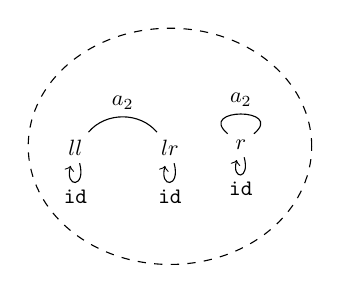
\begin{tikzpicture}[scale=0.6,every node/.style={scale=0.8}]
  \draw[dashed] (0,-0.3) ellipse (3cm and 2.5cm);
  \node[below] (A) at (-2,0) {$ll$};
  \node[below] (B) at (0,0) {$lr$};
  \node[below] (C) at (1.5,0) {$r$};
  \path (A) edge [bend left=50] node[above] {$a_2$} (B);
  \path (C) edge [out=140, in=40, looseness=4] node[above] {$a_2$}  (C);
  \path (A) edge [loop below] node[below] {\texttt{id}} (A);
  \path (B) edge [loop below] node[below] {\texttt{id}} (B);
  \path (C) edge [loop below] node[below] {\texttt{id}} (C);
\end{tikzpicture}
\end{center}

As explained above, the groupoid has cardinality $\frac{3}{2}$ which corresponds
to the quotient of the cardinality of the set $\mathbb{3}$ divided by the order
of $a_2$. This example groupoid is an instance of a groupoid construction known
as an \emph{action groupoid} explained next.

%%%%%%%%%%%%%%%%%%%%%%%
\subsection{Action Groupoids $\ag{\tau}{p}$}

Action groupoids~\cite{groupoidintro} were the inspiration for our
semantic development. They provide the main insight of using the
group structure associated with reversible programs as the equivalence
relation used to build quotient types. Once this construction was
thoroughly understood, it was generalized to iteration groupoids,
inverse order groupoids, and division groupoids that are actually used
in our semantics. We find it illuminating to present the material
starting from action groupoids.

Given a type $\tau$ and 1-combinator $p : \tau \iso \tau$, we build a
groupoid $\ag{\tau}{p}$ defined as follows. The objects of
$\ag{\tau}{p}$ are the elements~$v_i$ of the set $\sem{\tau}$ and there
is a morphism between $v_i$ and~$v_j$, if applying some number of
iterations of $p$ to $v_i$ produces~$v_j$. For example, consider the
type $\mathbb{3}$ and the 1-combinator $a_2$ from
Sec.~\ref{sec:pisem}. Since $a_2$ has order 2, we have that $a_2 ^ k$
for any integer~$k$ is, up to equivalence, either $\texttt{id}$ or
$a_2$. Therefore, the groupoid $\ag{\mathbb{3}}{a_2}$ looks exactly like
$G_2$ in Fig.~\ref{fig:groupoids2} with the names of the objects
relabeled to $\inl{(\inl{\unitv})}$, $\inl{(\inr{\unitv})}$, and
$\inr{\unitv}$ and the non-identity morphisms labeled $a_2$. As
explained above, the groupoid has cardinality $\frac{3}{2}$ which
corresponds to the quotient of the cardinality of the set $\mathbb{3}$
divided by the order of $a_2$. Note that in the calculation of
cardinality, we use the fact that the loop $a_2 \odot a_2$ going from
$\inl{(\inl{\unitv})}$ to $\inl{(\inr{\unitv})}$ and back is equivalent
to the identity.

Generally speaking, using known facts about the order of permutations
on finite sets, we highlight a few additional properties of action
groupoids. For a 1-combinator $p : \tau \iso \tau$, the cardinality of
$\ag{\tau}{p}$ is $|\tau|/\ord{p}$, i.e., the number of elements of
$\sem{\tau}$ divided by the order of the 1-combinator $p$.  For every
type $\tau$, including $\zt$, we can form the action groupoid
$\ag{\tau}{\idiso}$ whose cardinality is just the number of elements
in the set $\tau$. For any two types $\tau_1$ and $\tau_2$, we can
form the action groupoid $\ag{(\tau_1\oplus\tau_2)}{\swapp}$ whose
cardinality is half of the sum of the number of elements in $\tau_1$
and $\tau_2$. Given $p_1 : \tau_1 \iso \tau_1$ of order $o_1$ and
$p_2 : \tau_2 \iso \tau_2$ of order $o_2$, we can also form the action
groupoid $\ag{(\tau_1\oplus\tau_2)}({p_1\oplus p_2)}$ whose cardinality is
the sum of the elements $\tau_1$ and $\tau_2$ divided by the least
common multiple of $o_1$ and $o_2$. In case the cardinality of
$\tau_1$ is 3, the cardinality of $\tau_2$ is 2, the order of $p_1$ is
3, and the order of $p_2$ is 2, the resulting groupoid has cardinality
$\frac{5}{6}$ which is a proper fraction.

% \begin{center}
% \begin{tikzpicture}[scale=0.7,every node/.style={scale=0.8}]
%   \draw[dashed] (0,-0.3) ellipse (4.5cm and 2cm);
%   \node[below] (A) at (-3,0) {$\inl{(\inl{\unitv})}$};
%   \node[below] (B) at (0,0) {$\inl{(\inr{\unitv})}$};
%   \node[below] (C) at (3,0) {$\inr{\unitv}$};
%   \path (A) edge [bend left=50] node[above] {$a_2$} (B);
%   \path (C) edge [out=140, in=40, looseness=4] node[above] {$a_2$} (C);
%   \path (A) edge [loop below] node[below] {\texttt{id}} (A);
%   \path (B) edge [loop below] node[below] {\texttt{id}} (B);
%   \path (C) edge [loop below] node[below] {\texttt{id}} (C);
% \end{tikzpicture}
% \end{center}

\paragraph{Intermezzo.} Before concluding this section, we focus on
$G_2$ and how to compute its cardinality in an alternative,
compositional, way by viewing $G_2$ as being equivalent to the product
of two independent subsystems consisting of $\mathbb{3}$ and
$\iorder{a_2}$. Because the cardinality of $\mathbb{3}$ is 3 and the
final cardinality of $G_2$ is $\frac{3}{2}$, it must be that, using
$a_2$ to define $\iorder{a_2}$ produces a groupoid with
cardinality~$\frac{1}{2}$. From the information-theoretic perspective,
each state of the system represented by the type $\mathbb{3}$ has
$\log 3$ bits; after combining the type $\mathbb{3}$ with the type
$\iorder{a_2}$, the information contained in each state is reduced to
$\log \frac{3}{2} = \log 3 - \log 2$ bits. It must therefore be the case
that each state of the system represented by $\iorder{a_2}$ has a
negative amount of information $- \log 2 = \log \frac{1}{2}$ which
agrees with our observation that this use of $a_2$ must have cardinality
$\frac{1}{2}$. Intuitively speaking, imposing an equivalence relation on
a type translates as the inability to distinguish previously
distinguishable states. This indistinguishability subtracts knowledge
about the system and hence, when viewed as an independent system, must
have fractional cardinality.

%%%%%%%%%%%%%%%%%%%%%%%
\subsection{Program Iteration as Data}

Action groupoids $\ag{\tau}{p}$ allow us to build groupoids with
fractional cardinality by taking the quotient of a simple finite type
$\tau$ under the equivalence relation generated by an automorphism $p$
on $\tau$. We can generalize the situation by viewing $\ag{\tau}{p}$
as being formed from the product $\tau \otimes (\iorder{p})$
consisting a plain type $\tau$ and a ``pure'' equivalence relation
$\iorder{p}$. Before explaining the construction of $\iorder{p}$ we
will present the construction of a simpler related groupoid
$\order{p}$ that will serve as the multiplicative inverse of
$\iorder{p}$. Both constructions depend on the possibility of treating
programs (1-combinators) from a type to itself as data. More
precisely, for each 1-combinator $p : \tau\iso\tau$, we form the set
$\iter{p}$ whose elements are triples consisting of an integer $k$, a
1-combinator $q : \tau\iso\tau$ and a 2-combinator
$\alpha : q \isotwo p^k$.  For example, we have:
\[\begin{array}{rcl}
\iter{a_2} &=& \{ \triple{0}{\idiso}{\idisotwo},\triple{1}{a_2}{\idrdr}, \triple{-1}{a_2}{\idisotwo}, \ldots \}
\end{array}\]
The idea is that $\iter{a_2}$ is, up to equivalence, the set of all
distinct iterates $(a_2)^k$ of $a_2$.  Because of the underlying group
structure of automorphisms, there are, up to equivalence, only
$\ord{a_2}$ distinct iterates in $\iter{a_2}$.  We emphasize that, in
our proof-relevant setting, it is critical not to collapse
$\iter{a_2}$ to just $\{ \idiso, a_2 \}$. In the next two sections, we
will use the elements of $\iter{p}$ as either objects (emphasizing
their ``data'' aspect) or morphisms (emphasizing their ``program''
aspect) in various groupoid constructions.

%%%%%%%%%%%%%%%%%%%%%%%
\subsection{Iteration Groupoids $\order{p}$}

In the previous section, we collected the iterates of a 1-combinator
$p : \tau\iso\tau$ into a set $\iter{p}$ consisting of triples
$\triple{k}{q}{\alpha}$ indexed by integers $k$, 1-combinators
$q : \tau\iso\tau$, and 2-combinators $\alpha : q \isotwo p^k$. Not
all the iterates are independent, however. If $p$ has order $o$, then
the iterate $\triple{i}{q_i}{\alpha_i}$ and the iterate
$\triple{i+o}{q_j}{\alpha_j}$ must be equivalent in the sense that
there must be a 2-combinator relating $p^i \isotwo p^{i+o}$ and hence
$q_i \isotwo q_j$. If we add morphisms to witness equivalences between
iterates we get the groupoid $\order{p}$.

Formally, given a 1-combinator $p : \tau\iso\tau$, the groupoid
$\order{p}$ is the groupoid whose objects are the elements
$\triple{k}{q}{\alpha}$ of $\iter{p}$. There is a morphism between
$\triple{k_1}{q_1}{\alpha_1}$ and $\triple{k_2}{q_2}{\alpha_2}$ if
$q_1 \isotwo q_2$. (See Appendix for the Agda construction.)

\begin{lemma}
  $|\order{p}| = \ord{p}$
\end{lemma}
\begin{proof}
  Let $o = \ord{p}$. There are $o$ isomorphism classes of
  objects. Consider an object $x = \triple{k}{q}{\alpha}$, its
  isomorphism class $[x] = \triple{k+io}{q_i}{\alpha_i}$ where
  $i \in \Z$. The group $\textsf{Aut}(x)$ is the group generated by
  $\idisotwo$ and has order 1. Hence
  $|\order{p}| = \sum\limits_{1}^{o}\frac{1}{1} = o$.
\end{proof}

%%%%%%%%%%%%%%%%%%%%%%%
\subsection{Inverse Order Groupoids $\iorder{p}$}

The elements of $\iter{p}$ form a group under the following operation:
\[\begin{array}{l}
\triple{k_1}{p_1}{\alpha_1} ~\circ~ \triple{k_2}{p_2}{\alpha_2} = \\
\qquad  \triple{k_1+k_2}{p_1 \odot p_2}{(\alpha_1 ~\respstwo~
    \alpha_2)~\transtwo~(\distiterplus{p}{k_1}{k_2})}
\end{array}\]
where $\distiterplus{p}{k_1}{k_2}$ is defined in
Lem.~\ref{lem:distiterplus}. The common categorical representation of
a group is a category with one trivial object and the group elements
as morphisms on that trivial object. Our construction is essentially
the same except that the trivial object is represented as the iterates
of the identity over a singleton type.

Formally, given a 1-combinator $p : \tau\iso\tau$, the groupoid
$\iorder{p}$ is the groupoid (2-groupoid technically) whose objects
are the iterates in $\iter{\idiso_{\top}}$. Every pair of objects is
connected by the morphisms in $\iter{p}$. To capture the relationship
between these morphisms, we also have 2-morphisms relating the
distinct iterates as in the previous section. (See Appendix for the
Agda construction.)

\begin{lemma}
  $|\iorder{p}| = \frac{1}{\ord{p}}$
\end{lemma}
\begin{proof}
  Let $o = \ord{p}$. The objects form one isomorphism class
  $[p]$. There are, up to equivalence, exactly $\ord{p}$ distinct
  morphisms on this equivalence class. Hence, the group
  $\textsf{Aut}([p])$ is the group generated by
  $p^0, p^1 \dots p^{o-1}$, and the cardinality $|\iorder{p}|$ is
  $\frac{1}{o}$.
\end{proof}

Note that for each power $p ^ i$ of $p$, there is a morphism
$\triple{k}{q}{\alpha}$ in $\iter{p}$ such that $q$ annihilates $p^i$
to the identity. Note also that everything is well-defined even if we
choose $p : \zt\iso\zt$. In that case, the cardinality is 1.

%%%%%%%%%%%%%%%%%%%%%%%
\subsection{Division Groupoids $\divg{p}{r}$}

The groupoid $\order{p}$ can be thought of as
$\divg{p}{\idiso}$. Similarly the groupoid $\iorder{p}$ can be thought
of as $\divg{\idiso}{p}$. The two previous constructions can therefore
be generalized to allow arbitrary combinators in both the numerator
and denominator.

Formally, given two 1-combinators $p, r : \tau\iso\tau$, the objects
of $\divg{p}{r}$ are all the iterates $\iter{p}$, the numerator. There
is a morphism between $\triple{k_1}{q_1}{\alpha_1}$ and
$\triple{k_2}{q_2}{\alpha_2}$ if there exists an iterate
$\triple{k}{q}{\alpha}$ in $\iter{r}$, the denominator, such that
$(q_1 \odot q) \isotwo (q \odot q_2)$. As before, the morphisms are
not all independent: two morphisms are identified if their $q$
components are related by $\isotwo$.

When $r$ is $\idiso$, this construction reduces to $\order{p}$. When $p$
is $\idiso$, this construction reduces to $\iorder{r}$. Generally, the
cardinality of $\divg{p}{r}$ is $\frac{\ord{p}}{\ord{r}}$. (See Appendix
for the Agda construction.)


% %%%%%%%%%%%%%%%%%%%%%%%
% \subsection{Expanded Unit Groupoids $\oneg{p}$}

% For each combinator $p : \tau\iso\tau$, we also construct a groupoid
% $\oneg{p}$ of cardinality $\frac{\ord{p}}{\ord{p}} = 1$. (Recall that
% the order of a combinator can never be 0.) The objects of this
% groupoid as the iterates in $\iter{p}$. There is morphism between
% $\triple{k_1}{q_1}{\alpha_1}$ and $\triple{k_2}{q_2}{\alpha_2}$ if
% there exists a $\triple{k}{q}{\alpha}$ such that $q_1 ~\odot~ !q_2
% \isotwo q$.

%%%%%%%%%%%%%
\subsection{Groupoid of Groupoids}

The individual groupoids denoted by the types are themselves objects
in a larger groupoid. Formally, the language $\Pi$ models what is
called a \emph{symmetric bimonoidal category} or a \emph{commutative
  rig category}. These are categories with two binary operations and
satisfying the axioms of a commutative rig (i.e., a commutative ring
without negative elements, also known as a commutative semiring) up to
coherent isomorphisms. And indeed the types of the $\Pi$ 1-combinators
are precisely the commutative semiring axioms. A formal way of saying
this is that $\Pi$ is the \emph{categorification}~\cite{math/9802029}
of the natural numbers.

As suggested above, a simple (slightly degenerate) example of such
categories is the category of finite sets and permutations in which we
interpret every $\Pi$-type as a finite set, interpret the values as
elements in these finite sets, and interpret the 1-combinators as
permutations. More generally, the types of $\Pi$ are objects that
model sets of natural numbers, the 1-combinators are morphisms that
model cardinality-preserving maps, and the 2-combinators are coherence
conditions on these morphisms~\cite{Carette2016}. The resulting
$\Pi$-category has a rich structure consisting of two symmetric
monoidal structures~\cite{nla.cat-vn1051288} separately induced by the
properties of addition and multiplication of the natural
numbers. These two structures are then augmented with distributivity
and absorption natural isomorphisms~\cite{laplaza} to model the full
commutative semiring (aka, commutative rig) of the natural
numbers. All the morphisms are invertible which makes the resulting
category a ``symmetric rig groupoid''~\cite{nlabrig}.

Despite this rich structure, the individual objects in the category
for $\Pi$ are just plain sets with no interesting structure. With the
addition of action groupoids, iteration groupoids, inverse order
groupoids, and division groupoids we can enrich the symmetric rig
groupoid of $\Pi$ so that objects themselves carry a non-trivial
groupoid structure. Sums and products of these groupoids behave as
expected which ensures that a sensible compositional programming
language can be designed around fractional types. This is the subject
of next section.

%% Talk about monad/comonad ????

% %%%%%
% \subsection{Old stuff to clean up or throw away}

% \amr{from popl 12 paper: adapt}

% We want our computations to be information-preserving. Since the
% amount of information in each state is just the log of the cardinality
% of the space, computation just needs to be between spaces of the same
% cardinality.

%  Now consider the \ensuremath{\mathit{bool} \rightarrow \mathit{bool}}
% function \ensuremath{\mathit{not}}. Let $p_F$ and $p_T$ be the
% probabilities that the input is \ensuremath{\mathit{false}} or
% \ensuremath{\mathit{true}} respectively. The outputs occur with the
% reverse probabilities, i.e., $p_T$ is the probability that the output
% is \ensuremath{\mathit{false}} and $p_F$ is the probability that t he
% output is \ensuremath{\mathit{true}}. Hence the output entropy of the
% function is $- p_F \log{p_F} - p_T \log{p_T}$ which is the same as the
% input entropy and the function is information-preserving. As another
% example, consider the \ensuremath{\mathit{bool} \rightarrow
%   \mathit{bool}} function \ensuremath{\mathit{constT}(x) =
%   \mathit{true}} which discards its input.  The output of the function
% is always \ensuremath{\mathit{true}} with no uncertainty, which means
% tha t the output entropy is 0, and that the function is not
% information-preserving. As a third example, consider the
% function~\ensuremath{\mathit{and}} and let the inputs occur with equal
% probabilities, i.e., let the entropy of the input be 2. The output is
% \ensuremath{\mathit{false}} with probability $3/4$ and
% \ensuremath{\mathit{true}} with probability $1/4$, which means that
% the output entropy is about 0.8 and the function is not
% information-preserving. As a final example, consider the
% \ensuremath{\mathit{bool} \rightarrow \mathit{bool}\times
%   \mathit{bool}} function \ensuremath{\mathit{fanout} ~(x) = (x,x)}
% which duplicates its input.  Let the input be
% \ensuremath{\mathit{false}} with probability $p_F$ and
% \ensuremath{\mathit{true}} be probability $p_T$. The output is
% \ensuremath{(\mathit{false},\mathit{false})} with probability $p_F$
% and \ensuremath{(\mathit{true},\mathit{true})} with probability $p_T$
% which means that the output entropy is the same as the input entropy
% and the function is information-preserving.

% We are now ready to formalize the connection between reversibility and
% entropy, once we define logical reversibility of computations.

% \begin{definition}[Logical reversibility~\cite{Zuliani:2001:LR}]
% A function $f : b_1 \rightarrow b_2$ is logically reversible if there exists
% an inverse function $g : b_2 \rightarrow b_1$ such that for all values $v_1
% \in b_1$ and $v_2 \in b_2$, we have: $f(v_1) = v_2$ iff $g(v_2) = v_1$.
% \end{definition}

% \noindent The main proposition that motivates and justifies our approach is that
% logically reversible functions are information-preserving.

% \begin{proposition}
% A function is logically reversible iff it is information-preserving.
% \end{proposition}

% Looking at the examples above, we argued that \ensuremath{\mathit{constT}}, \ensuremath{\mathit{and}} are
% not information-preserving and that \ensuremath{\mathit{not}}, \ensuremath{\mathit{fanout}} are
% information-preserving. As expected, neither \ensuremath{\mathit{constT}} nor \ensuremath{\mathit{and}}
% are logically reversible and \ensuremath{\mathit{not}} is logically reversible. The
% situation with \ensuremath{\mathit{fanout}} is however subtle and deserves some
% explanation. First, note that the definition of logical reversibility
% does not require the functions to be total, and hence it is possible
% to define a \emph{partial} function \ensuremath{\mathit{fanin}} that is the logical
% inverse of \ensuremath{\mathit{fanout}}. The function \ensuremath{\mathit{fanin}} maps \ensuremath{(\mathit{false},\mathit{false})}
% to \ensuremath{\mathit{false}}, \ensuremath{(\mathit{true},\mathit{true})} to \ensuremath{\mathit{true}} and is undefined
% otherwise. Arguing that partial functions like \ensuremath{\mathit{fanin}} are
% information-preserving requires some care. Let the inputs to \ensuremath{\mathit{fanin}}
% occur with equal probabilities, i.e., let the entropy of the input
% be~2. Disregarding the partiality of \ensuremath{\mathit{fanin}}, one might reason that
% the output is \ensuremath{\mathit{false}} with probability $1/4$ and \ensuremath{\mathit{true}} with
% probability $1/4$ and hence that the output entropy is~1 which
% contradicts the fact that \ensuremath{\mathit{fanin}} is logically reversible. The
% subtlety is that entropy is defined with respect to observing some
% probabilistic event: an infinite loop is not an event that can be
% observed and hence the entropy analysis, just like the definition of
% logical reversibility, only applies to the pairs of inputs and outputs
% on which the function is defined. In the case of \ensuremath{\mathit{fanin}} this means
% that the only inputs that can be considered are \ensuremath{(\mathit{false},\mathit{false})} and
% \ensuremath{(\mathit{true},\mathit{true})} and in this case it is clear that the function is
% information-preserving as expected.

% \amr{end of popl 12 quote}

% %%%%%
% \subsection{Constraints}

% If we have the type $\mathsf{Bool} \times \mathsf{Bool}$ the
% information in each state is 2 bits. But if our system also has a
% constraint that the state must be of the form $(b,b)$, then there are
% only possible states in the system and the information contained in
% each is just one bit. There is a neat way to express the constraint
% using an equivalence generated by a pi-program.

% %%%%%
% \subsection{Information Equivalence}

% We need to show coherence of the definition of cardinalities on the
% universe syntax with the Euler characteristic of the category which in
% our case also corresponds to the groupoid cardinality. There are
% several formulations and explanations. The following is quite simple
% to implement: first collapse all the isomorphic objects. Then fix a
% particular order of the objects and write a matrix whose $ij$'s entry
% is the number of morphisms from $i$ to $j$. Invert the matrix. The
% cardinality is the sum of the elements in the matrix.

% Our notion of information equivalence is coarser than the conventional
% notion of equivalence of categories (groupoids). This is fine as there
% are several competing notions of equivalence of groupoids that are
% coarser than strict categorical equivalence.

% There are however other notions of equivalence of groupoids like
% Morita equivalence and weak equivalence that we explore later. The
% intuition of these weaker notions of equivalence is that two groupoids
% can be considered equivalent if it is not possible to distinguish them
% using certain observations. This informally corresponds to the notion
% of ``observational equivalence'' in programming language
% semantics. Note that negative entropy can only make sense locally in
% an open system but that in a closed system, i.e., in a complete
% computation, entropy cannot be negative. Thus we restrict
% observational contexts to those in which fractional types do not
% occur. Note that two categories can have the same cardinality but not
% be equivalent or even Morita equivalent but the converse is
% guaranteed. So it is necessary to have a separate notion of
% equivalence and check that whenever we have the same cardinality, the
% particular categories in question are equivalent.

% \begin{code}
% -- Conjecture:  p ⇔ q   implies  order p = order q
% -- Corollary:   p ⇔ !q  implies  order p = order (! q)

% -- The opposite is not true.

% -- Example
% -- p = (1 2 3 4)

% -- compose p 0 = compose !p 0 = compose p 4 = compose !p 4
% -- 1 -> 1
% -- 2 -> 2
% -- 3 -> 3
% -- 4 -> 4

% -- compose p 1  ***     compose !p 1
% -- 1 -> 2       ***     1 -> 4
% -- 2 -> 3       ***     2 -> 1
% -- 3 -> 4       ***     3 -> 2
% -- 4 -> 1       ***     4 -> 3

% -- compose p 2  ***     compose !p 2
% -- 1 -> 3       ***     1 -> 3
% -- 2 -> 4       ***     2 -> 4
% -- 3 -> 1       ***     3 -> 1
% -- 4 -> 2       ***     4 -> 2

% -- compose p 3  ***     compose !p 3
% -- 1 -> 4       ***     1 -> 2
% -- 2 -> 1       ***     2 -> 3
% -- 3 -> 2       ***     3 -> 4
% -- 4 -> 3       ***     4 -> 1

% -- there is a morphism 1 -> 2 using
% -- (compose p 1) and (compose !p 3)
% -- p¹ is the same as !p³
% -- p² is the same as !p²
% -- p³ is the same as !p¹

% data FT/ : Set where
%   ⇑    : FT → FT/
%   #    : {τ : FT} → (p : τ ⟷ τ) → FT/
%   1/#  : {τ : FT} → (p : τ ⟷ τ) → FT/
%   _⊞_  : FT/ → FT/ → FT/
%   _⊠_  : FT/ → FT/ → FT/

% UG : Universe l0 (lsuc l0)
% UG = record {
%     U = FT/
%  ;  El = λ T → Σ[ ℂ ∈ Category l0 l0 l0 ] (Groupoid ℂ)
%  }

% card : FT/ → ℚ
% card (⇑ τ)      = mkRational ∣ τ ∣ 1 {tt}
% card (# p)      = mkRational (order p) 1 {tt}
% card (1/# p)    = mkRational 1 (order p) {order-nz}
% card (T₁ ⊞ T₂)  = (card T₁) ℚ+ (card T₂)
% card (T₁ ⊠ T₂)  = (card T₁) ℚ* (card T₂)
% \end{code}

% %%%%%
% \subsection{Groupoids from $\Pi$-Combinators}

% The goal is to define a function that takes a $T$ in $FT/$ and
% produces something of type $Universe.El~UG~T$, i.e., a particular
% groupoid.

% \begin{code}

% -- First each p is an Agda type
% -- Perm p i is the type that contains the i^th iterate
% -- of p, i.e p^i up to <=>.
% -- the parens in the definition of ^ need to be there!

% _^_ : {τ : FT} → (p : τ ⟷ τ) → (k : ℤ) → (τ ⟷ τ)
% p ^ (+ 0) = id⟷
% p ^ (+ (suc k)) = p ◎ (p ^ (+ k))
% p ^ -[1+ 0 ] = ! p
% p ^ (-[1+ (suc k) ]) = (! p) ◎ (p ^ -[1+ k ])

% -- i.e. Perm is: for all i, any p' such that
% -- p' ⇔ p ^ i

% record Perm {τ : FT} (p : τ ⟷ τ) : Set where
%   constructor perm
%   field
%     iter : ℤ
%     p' : τ ⟷ τ
%     p'⇔p^i : p' ⇔ p ^ iter

% cong^ : {τ : FT} → {p q : τ ⟷ τ} → (k : ℤ) → (eq : p ⇔ q) →
%   p ^ k ⇔ q ^ k
% cong^ (+_ ℕ.zero) eq = id⇔
% cong^ (+_ (suc n)) eq = eq ⊡ cong^ (+ n) eq
% cong^ (-[1+_] ℕ.zero) eq = ⇔! eq
% cong^ (-[1+_] (suc n)) eq = (⇔! eq) ⊡ cong^ (-[1+ n ]) eq

% -- this should go into PiLevel1

% !!⇔id : {t₁ t₂ : FT} → (p : t₁ ⟷ t₂) → p ⇔ ! (! p)
% !!⇔id _⟷_.unite₊l = id⇔
% !!⇔id _⟷_.uniti₊l = id⇔
% !!⇔id _⟷_.unite₊r = id⇔
% !!⇔id _⟷_.uniti₊r = id⇔
% !!⇔id _⟷_.swap₊ = id⇔
% !!⇔id _⟷_.assocl₊ = id⇔
% !!⇔id _⟷_.assocr₊ = id⇔
% !!⇔id _⟷_.unite⋆l = id⇔
% !!⇔id _⟷_.uniti⋆l = id⇔
% !!⇔id _⟷_.unite⋆r = id⇔
% !!⇔id _⟷_.uniti⋆r = id⇔
% !!⇔id _⟷_.swap⋆ = id⇔
% !!⇔id _⟷_.assocl⋆ = id⇔
% !!⇔id _⟷_.assocr⋆ = id⇔
% !!⇔id _⟷_.absorbr = id⇔
% !!⇔id _⟷_.absorbl = id⇔
% !!⇔id _⟷_.factorzr = id⇔
% !!⇔id _⟷_.factorzl = id⇔
% !!⇔id _⟷_.dist = id⇔
% !!⇔id _⟷_.factor = id⇔
% !!⇔id _⟷_.distl = id⇔
% !!⇔id _⟷_.factorl = id⇔
% !!⇔id id⟷ = id⇔
% !!⇔id (p ◎ q) = !!⇔id p ⊡ !!⇔id q
% !!⇔id (p _⟷_.⊕ q) = resp⊕⇔ (!!⇔id p) (!!⇔id q)
% !!⇔id (p _⟷_.⊗ q) = resp⊗⇔ (!!⇔id p) (!!⇔id q)

% -- because ^ is iterated composition of the same thing,
% -- then by associativity, we can hive off compositions
% -- from left or right

% assoc1 : {τ : FT} → {p : τ ⟷ τ} → (m : ℕ) →
%   (p ◎ (p ^ (+ m))) ⇔ ((p ^ (+ m)) ◎ p)
% assoc1 ℕ.zero = trans⇔ idr◎l idl◎r
% assoc1 (suc m) = trans⇔ (id⇔ ⊡ assoc1 m) assoc◎l

% assoc1- : {τ : FT} → {p : τ ⟷ τ} → (m : ℕ) →
%   ((! p) ◎ (p ^ -[1+ m ])) ⇔ ((p ^ -[1+ m ]) ◎ (! p))
% assoc1- ℕ.zero = id⇔
% assoc1- (suc m) = trans⇔ (id⇔ ⊡ assoc1- m) assoc◎l

% -- Property of ^: negating exponent is same as
% -- composing in the other direction, then reversing.
% ^⇔! : {τ : FT} → {p : τ ⟷ τ} → (k : ℤ) →
%   (p ^ (ℤ- k)) ⇔ ! (p ^ k)
% ^⇔! (+_ ℕ.zero) = id⇔
% -- need to dig deeper, as we end up negating
% ^⇔! (+_ (suc ℕ.zero)) = idl◎r
% ^⇔! (+_ (suc (suc n))) = trans⇔ (assoc1- n) (^⇔! (+ suc n) ⊡ id⇔)
% ^⇔! {p = p} (-[1+_] ℕ.zero) = trans⇔ idr◎l (!!⇔id p)
% ^⇔! {p = p} (-[1+_] (suc n)) =
%   trans⇔ (assoc1 (suc n)) ((^⇔! -[1+ n ]) ⊡ (!!⇔id p))

% -- first match on m, n, then proof is purely PiLevel1
% lower : {τ : FT} {p : τ ⟷ τ} (m n : ℤ) →
%   p ^ (m ℤ+ n) ⇔ ((p ^ m) ◎ (p ^ n))
% lower (+_ ℕ.zero) (+_ n) = idl◎r
% lower (+_ ℕ.zero) (-[1+_] n) = idl◎r
% lower (+_ (suc m)) (+_ n) =
%   trans⇔ (id⇔ ⊡ lower (+ m) (+ n)) assoc◎l
% lower {p = p} (+_ (suc m)) (-[1+_] ℕ.zero) =
%   trans⇔ idr◎r (trans⇔ (id⇔ ⊡ linv◎r) (
%   trans⇔ assoc◎l (2! (assoc1 m) ⊡ id⇔)))  -- p ^ ((m + 1) -1)
% lower (+_ (suc m)) (-[1+_] (suc n)) = -- p ^ ((m + 1) -(1+1+n)
%   trans⇔ (lower (+ m) (-[1+ n ])) (
%   trans⇔ ((trans⇔ idr◎r (id⇔ ⊡ linv◎r))  ⊡ id⇔) (
%   trans⇔ assoc◎r (trans⇔ (id⇔ ⊡ assoc◎r) (
%   trans⇔ assoc◎l (2! (assoc1 m) ⊡ id⇔)))))
% lower (-[1+_] m) (+_ ℕ.zero) = idr◎r
% lower (-[1+_] ℕ.zero) (+_ (suc n)) = 2! (trans⇔ assoc◎l (
%   trans⇔ (rinv◎l ⊡ id⇔) idl◎l))
% lower (-[1+_] (suc m)) (+_ (suc n)) = -- p ^ (-(1+m) + (n+1))
%   trans⇔ (lower (-[1+ m ]) (+ n)) (
%     trans⇔ ((trans⇔ idr◎r (id⇔ ⊡ rinv◎r))  ⊡ id⇔) (
%   trans⇔ assoc◎r (trans⇔ (id⇔ ⊡ assoc◎r) (
%   trans⇔ assoc◎l ((2! (assoc1- m)) ⊡ id⇔)))))
% lower (-[1+_] ℕ.zero) (-[1+_] n) = id⇔
% lower (-[1+_] (suc m)) (-[1+_] n) = -- p ^ (-(1+1+m) - (1+n))
%   trans⇔ (id⇔ ⊡ lower (-[1+ m ]) (-[1+ n ])) assoc◎l


% -- orderC is the groupoid with objects p^i

% orderC : {τ : FT} → (p : τ ⟷ τ) → Category _ _ _
% orderC {τ} p = record {
%      Obj = Perm p
%    ; _⇒_ = λ { (perm i p₁ _) (perm j p₂ _) → p₁ ⇔ p₂ }
%    ; _≡_ = λ _ _ → ⊤
%    ; id = id⇔
%    ; _∘_ = λ α β → trans⇔ β α
%    ; assoc = tt
%    ; identityˡ = tt
%    ; identityʳ = tt
%    ; equiv = record { refl = tt; sym = λ _ → tt; trans = λ _ _ → tt }
%    ; ∘-resp-≡ = λ _ _ → tt
%    }
%    where open Perm

% orderG : {τ : FT} → (p : τ ⟷ τ) → Groupoid (orderC p)
% orderG {τ} p = record {
%     _⁻¹ = 2!
%   ; iso = record {
%         isoˡ = tt
%       ; isoʳ = tt
%       }
%   }

% -- discrete groupoids corresponding to plain pi types

% discreteC : Set → Category _ _ _
% discreteC S = record {
%      Obj = S
%     ; _⇒_ = _≡_
%     ; _≡_ = λ _ _ → ⊤
%     ; id = refl
%     ; _∘_ = λ { {A} {.A} {.A} refl refl → refl }
%     ; assoc = tt
%     ; identityˡ = tt
%     ; identityʳ = tt
%     ; equiv = record { refl = tt; sym = λ _ → tt; trans = λ _ _ → tt }
%     ; ∘-resp-≡ = λ _ _ → tt
%     }

% discreteG : (S : Set) → Groupoid (discreteC S)
% discreteG S = record
%   { _⁻¹ = λ { {A} {.A} refl → refl }
%   ; iso = record { isoˡ = tt; isoʳ = tt }
%   }

% -- fractional groupoid

% 1/orderC : {τ : FT} (p : τ ⟷ τ) → Category _ _ _
% 1/orderC {τ} pp = record {
%      Obj = ⊤
%     ; _⇒_ = λ _ _ → Perm pp
%     ; _≡_ = λ { (perm m p _) (perm n q  _) → p ⇔ q } -- pp ^ m ⇔ pp ^ n
%     ; id = perm (+ 0) id⟷ id⇔
%     ; _∘_ = λ { (perm m p α) (perm n q β) →
%         perm (m ℤ+ n) (p ◎ q) (trans⇔ (α ⊡ β) (2! (lower m n))) }
%     ; assoc = assoc◎r
%     ; identityˡ = idl◎l
%     ; identityʳ =  idr◎l
%     ; equiv = record { refl = id⇔; sym = 2!; trans = trans⇔ }
%     ; ∘-resp-≡ = _⊡_
%     }

% 1/orderG : {τ : FT} (p : τ ⟷ τ) → Groupoid (1/orderC p)
% 1/orderG p = record {
%       _⁻¹ = λ { (perm i q eq) →
%               perm (ℤ- i) (! q) (trans⇔ (⇔! eq) (2! (^⇔! {p = p} i)))}
%     ; iso = record { isoˡ = rinv◎l ; isoʳ = linv◎l }
%     }
% \end{code}

% %% _//_ : (τ : FT) → (p : τ ⟷ τ) → Category _ _ _
% %% τ // p = Product (discreteC (El τ)) (1/orderC p)
% %%   where open Universe.Universe UFT
% %%
% %% quotientG : (τ : FT) → (p : τ ⟷ τ) → Groupoid (τ // p)
% %% quotientG = {!!}

% So now we can finally define our denotations:

% \begin{code}
% ⟦_⟧/ : (T : FT/) → Universe.El UG T
% ⟦ ⇑ S ⟧/ = , discreteG (Universe.El UFT S)
% ⟦ # p ⟧/ = , orderG p
% ⟦ 1/# p ⟧/ = , 1/orderG p
% ⟦ T₁ ⊞ T₂ ⟧/ with ⟦ T₁ ⟧/ | ⟦ T₂ ⟧/
% ... | (_ , G₁) | (_ , G₂) = , GSum G₁ G₂
% ⟦ T₁ ⊠ T₂ ⟧/ with ⟦ T₁ ⟧/ | ⟦ T₂ ⟧/
% ... | (_ , G₁) | (_ , G₂) = , GProduct G₁ G₂
% \end{code}

%%%%%%%%%%%%%%%%%%%%%%%%%%%%%%%%%%%%%%%%%%%%%%%%%%%%%%%%%%%%%%%%%%%%%%%%%%%%%%

% -- p is a monad on (order p)

% ^suc : {τ : FT} {p : τ ⟷ τ} {i : ℤ} → p ^ ℤsuc i ⇔ p ◎ p ^ i
% ^suc = {!!}

% ^resp : {τ : FT} {p q : τ ⟷ τ} {i : ℤ} → (q ^ i ⇔ p ^ i) → (q ◎ q ^ i ⇔ p ◎ p ^ i)
% ^resp = {!!}

% orderM : {τ : FT} → (p : τ ⟷ τ) → Monad (orderC p)
% orderM {τ} p = record {
%     F = record {
%           F₀ = λ { (i , (q , α)) →
%                  (ℤsuc i , (q , trans⇔ (^suc {p = q} {i = i})
%                                 (trans⇔ (^resp {p = p} {q = q} {i = i} α)
%                                 (2! (^suc {p = p} {i = i})))))}
%         ; F₁ = {!!}
%         }
%   ; η = record {
%           η = {!!}
%         ; commute = λ _ → tt
%         }
%   ; μ = record {
%           η = {!!}
%         ; commute = λ _ → tt
%         }
%   ; assoc = tt
%   ; identityˡ = tt
%   ; identityʳ = tt
%   }

% -- ! p is a comonad on (order p)

% orderCom : {τ : FT} → (p : τ ⟷ τ) → Comonad (orderC p)
% orderCom {τ} p = record {
%     F = record {
%           F₀ = {!!}
%         ; F₁ = {!!}
%         }
%   ; η = record {
%           η = {!!}
%         ; commute = λ _ → tt
%         }
%   ; μ = record {
%           η = {!!}
%         ; commute = λ _ → tt
%         }
%   ; assoc = tt
%   ; identityˡ = tt
%   ; identityʳ = tt
%   }

% -- the monad and comonad are inverses
% -- idea regarding the significance of the
% -- monad/comonad construction. Say we have
% -- a combinator c : #p ⟷ #q that maps
% -- p^i to q^j. Then we can use the q-monad
% -- to write a combinator pc : #p ⟷ #q which
% -- maps p^i to q^j using c and then to
% -- q^(suc j) using the monad. We can use
% -- the comonad to map p^i to p^(suc i) and
% -- then to #q using c. So as an effect we can
% -- construct maps that move around #p and #q
% -- using p and q.
% --
% -- A more general perspective: computations
% -- happen in a context in the following sense:
% -- say we have a collection of values v1, v2, ...
% -- a computation takes vi to wi. In many cases,
% -- the vi's form a structure of some kind and
% -- so do the wi's. A monad focuses on the w's
% -- structure and how to compose computations
% -- on it. The comonad focuses on the v's structure
% -- and how to compose computations on it. Some
% -- people talk about monads expressing how to
% -- affect the context and comonads expressing
% -- what to expect from the context.

% -- moncom = ?

% -- 1/orderC is the the groupoid with one object
% --   and morphisms p^i

% 1/orderM : {τ : FT} (p : τ ⟷ τ) → Monad (1/orderC p)
% 1/orderM = {!!}

% 1/orderCom : {τ : FT} (p : τ ⟷ τ) → Comonad (1/orderC p)
% 1/orderCom = {!!}

% The definition of $p$ will induce three types (groupoids):

% \begin{itemize}

% \item The first is the action groupoid $\ag{C}{p}$ depicted below. The
% objects are the elements of $C$ and there is a morphism between $x$
% and $y$ iff $p^k$ for some $k$ maps $x$ to $y$. We do not draw the
% identity morphisms. Note that all of $p^0$, $p^1$, and $p^2$ map
% \texttt{sat} to \texttt{sat} which explains the two non-trivial
% morphisms on \texttt{sat}:

% \begin{center}
% \begin{tikzpicture}[scale=0.4,every node/.style={scale=0.4}]
%   \draw (0,0) ellipse (8cm and 1.6cm);
%   \node[below] at (-6,0) {\texttt{sun}};
%   \node[below] at (-4,0) {\texttt{mon}};
%   \node[below] at (-2,0) {\texttt{tue}};
%   \node[below] at (0,0) {\texttt{wed}};
%   \node[below] at (2,0) {\texttt{thu}};
%   \node[below] at (4,0) {\texttt{fri}};
%   \node[below] (B) at (6,0) {\texttt{sat}};
%   \draw[fill] (-6,0) circle [radius=0.05];
%   \draw[fill] (-4,0) circle [radius=0.05];
%   \draw[fill] (-2,0) circle [radius=0.05];
%   \draw[fill] (0,0) circle [radius=0.05];
%   \draw[fill] (2,0) circle [radius=0.05];
%   \draw[fill] (4,0) circle [radius=0.05];
%   \draw[fill] (6,0) circle [radius=0.05];
%   \draw (-6,0) -- (-4,0);
%   \draw (-4,0) -- (-2,0);
%   \draw (0,0) -- (2,0);
%   \draw (2,0) -- (4,0);
%   \draw (-6,0) to[bend left] (-2,0) ;
%   \draw (0,0) to[bend left] (4,0) ;
%   \path (B) edge [loop above, looseness=3, in=48, out=132] node[above] {} (B);
%   \path (B) edge [loop above, looseness=5, in=40, out=140] node[above] {} (B);
% \end{tikzpicture}
% \end{center}

% To calculate the cardinality, we first collapse all the isomorphic
% objects (i.e., collapse the two strongly connected components to one
% object each) and write the resulting matrix:
% \[
% \begin{pmatrix}
% 1 & 0 & 0 \\
% 0 & 1 & 0 \\
% 0 & 0 & 3
% \end{pmatrix}
% \]
% Its inverse is 0 everywhere except on the main diagonal which has
% entries 1, 1, and $\frac{1}{3}$ and hence the cardinality of this
% category is $2\frac{1}{3}$.

% \item The second which we call $1/p$ is depicted below. It has one
% trivial object and a morphism for each iteration of $p$. It has
% cardinality $\frac{1}{3}$ as the connectivity matrix has one entry
% $3$ whose inverse is $\frac{1}{3}$:

% \begin{center}
% \begin{tikzpicture}[scale=0.7,every node/.style={scale=0.8}]
%   \draw (0,1.4) ellipse (2cm and 2cm);
%   \node[below] (B) at (0,0) {\texttt{*}};
% %%  \path (B) edge [loop above] node[above] {$p^0$} (B);
%   \path (B) edge [loop above, looseness=15, in=48, out=132] node[above] {$p$} (B);
%   \path (B) edge [loop above, looseness=25, in=40, out=140] node[above] {$p^2$} (B);
% \end{tikzpicture}
% \end{center}

% \item The third is the order type $\order{p}$ depicted below. It has
% three objects corresponding to each iteration of $p$. It has
% cardinality $3$:
% \begin{center}
% \begin{tikzpicture}[scale=0.7,every node/.style={scale=0.8}]
%   \draw (0,0) ellipse (4cm and 1cm);
%   \node[below] at (-2,0) {$p^0$};
%   \node[below] at (0,0) {$p^1$};
%   \node[below] at (2,0) {$p^2$};
%   \draw[fill] (-2,0) circle [radius=0.05];
%   \draw[fill] (0,0) circle [radius=0.05];
%   \draw[fill] (2,0) circle [radius=0.05];
% \end{tikzpicture}
% \end{center}
% \end{itemize}

% Each combinator $p : \tau ⟷ \tau$ will give rise to two groupoids:
% \begin{itemize}
% \item one groupoid $\mathit{order}~p$ with objects $p^i$ and morphisms $⇔$, and
% \item another groupoid $\mathit{1/order}~p$ with one object and morphisms $p^i$ under $⇔$
% \end{itemize}
% There is also a third groupoid $\ag{\tau}{p}$ that is equivalent to
% $\tau \boxtimes \mathit{1/order}~p$ and that is a conventional quotient type.

% Is weak equivalence in HoTT related??? Here is one definition: A map
% $f : X \rightarrow Y$ is a weak homotopy equivalence (or just a weak
% equivalence) if for every $x \in X$, and all $n \geq 0$ the map
% $\pi_n(X,x) \rightarrow \pi_n(Y,f(x))$ is a bijection. In our setting
% this might mean something like: two types $T$ and $U$ are equivalent
% if $T \leftrightarrow T$ is equivalent to $U \leftrightarrow U$ are
% equivalent.

% -- These are true, but no longer used
% -- cancel-rinv : {τ : FT} → {p : τ ⟷ τ} → (i : ℤ) →
% --   ((p ^ i) ◎ ((! p) ^ i)) ⇔ id⟷
% -- cancel-rinv (+_ ℕ.zero) = idl◎l
% -- cancel-rinv (+_ (suc n)) =
% --   trans⇔ (assoc1 n ⊡ id⇔) (trans⇔ assoc◎l (trans⇔ (assoc◎r ⊡ id⇔)
% --   (trans⇔ ((id⇔ ⊡ linv◎l) ⊡ id⇔) (trans⇔ (idr◎l ⊡ id⇔) (
% --   cancel-rinv (+ n))))))
% -- cancel-rinv (-[1+_] ℕ.zero) = linv◎l
% -- cancel-rinv (-[1+_] (suc n)) =
% --   trans⇔ (assoc1- n ⊡ id⇔) (
% --   trans⇔ assoc◎l (trans⇔ (assoc◎r ⊡ id⇔)
% --   (trans⇔ ((id⇔ ⊡ linv◎l) ⊡ id⇔) (trans⇔ (idr◎l ⊡ id⇔)
% --   (cancel-rinv -[1+ n ])))))

% -- cancel-linv : {τ : FT} → {p : τ ⟷ τ} → (i : ℤ) →
% --   (((! p) ^ i) ◎ (p ^ i)) ⇔ id⟷
% -- cancel-linv (+_ ℕ.zero) = idr◎l
% -- cancel-linv (+_ (suc n)) = trans⇔ (assoc1 n ⊡ id⇔) (
% --    trans⇔ assoc◎l (trans⇔ (assoc◎r ⊡ id⇔) (
% --    trans⇔ ((id⇔ ⊡ rinv◎l) ⊡ id⇔) (trans⇔ (idr◎l ⊡ id⇔)
% --    (cancel-linv (+ n))))))
% -- cancel-linv (-[1+_] ℕ.zero) = rinv◎l
% -- cancel-linv (-[1+_] (suc n)) = trans⇔ (assoc1- n ⊡ id⇔) (
% --   trans⇔  assoc◎l (trans⇔ (assoc◎r ⊡ id⇔) (
% --   trans⇔ ((id⇔ ⊡ rinv◎l) ⊡ id⇔) (trans⇔ (idr◎l ⊡ id⇔) (
% --   cancel-linv -[1+ n ])))))

% one dollar and four quarters are indistinguishable because every
% transaction that can use one can use the other.

% v : obj, loop space
% loop : 1-combinator, 2 loop space
% 2-loop : 2-combinator

% define v ~ w; use any loop on v ...

%% can we show t // p has same values as t x 1/p

%% can we show 1 has same values as 3 x 1/3 which also has same values as
%% fully connected 3 points 3 // 3

%% -----------------

% Ok so let's say a is a value, b is a value, c is a value and we have
% the types

% a == a
% a == b
% a == c
% b == a
% b == b
% b == c
% c == a
% c == b
% c == c

% that we can use to reason about which values are equivalent to which
% values

% Some of these are inhabited: x == x always has refl, a == c has swap,
% c == a has swap, b == b has another member other than id which is swap
% a == b is empty and so on

%% -----------------

% First lemma: if x ==A y and c : A <-> B then eval(c,x) ==B eval(c,y)
% Proof: eval can manipulate the proof x == y along

% argue that it is awkward to carry all these equivalences around, so it
% is better to normalize everything and always manipulate fractional
% types of the form 1/x that way all the equivalences about a value are
% right there: we only have x == y iff x is identical to y but we may
% have many inhabitants of the space in that case

% so now a value is always of the form x as usual and then we have a
% bunch of identities x==x that we carry around with the value that are
% the cycles starting from x looping around and then coming back to x

% eta_p : produces (p,*) and the * has many equivalences *==* that are
% id,p,p2,p3,... epsilon receives (p,*) then all is good; epsilon
% receives (p2,*)

% Ok so perhaps we carry values and a list of transports to do; epsilon
% can just let (p2,*) go through but produce a transport along p2

% ---

% Main question: How do we argue that a system with one state is
% equivalent to a system with 3 states, each with with 1/3 information

% (*,id)

% vs

% (id,[id,p,p2]), (p,[id,p,p2]), (p2,[id,p,p2])

% ==>

% general idea

% (p,[...,q,...]) is indistinguishable from (q.p,[...,q.q,...])

% and

% (v,[id,p]) is indistinguishable from (ap p v, [ p , p2 ])

% So for example groupoid, we have the following values:

% (a,[id,swap])
% (b,[id,swap])
% (c,[id,swap])

% and (a,[id,swap]) ~id~ (a,[id,swap])
%       (a,[id,swap]) ~swap~ (c,[swap,swap2])
%       (b,[id,swap]) ~id~ (b,[id,swap])
%       (b,[id,swap]) ~swap~ (b,[swap,id])

% So now a value is (obj,[autos]) and we have ==G that tells us which
% values are indistinguishable from each other

% Back to eta/epsilon. Let p have order 3 for this example:

% eta_p (*,[id]) ==> ((p^1,*),([id],[id,p,p2]))

% epsilon_p ((p^i,*),([id],[id,p,p2]))

% No want:
% eta_p (*,[id]) ==> (id,[id,p,p2]) which is indistinguishable from (p,[id,p,p2]) and (p2,[id,p,p2])

% So a value is an object and a collection of loops
% A loop is a 1-combinator and a collection of 2-loops
% A 2-loop is a 2-combinator

% we have an equivalence relation on values telling us which values are
% indistinguishable; basically (v,[...p..]) is indistinguishable from
% (pv,[...p2,...]). Same with loops (p,[...alpha...]) is
% indistinguishable from (alpha p,[... alpha^2...])

% we have an equivalence between the type 1 viewed as (*,[id]) and
% viewed as { (id,[id,p,p2]), (p,[id,p,p2]), (p2,[id,p,p2]) }. The
% latter has 3 values but they are all indistinguishable so they are
% really one value. Eta allows us to separate one of the values in the
% second representation into two components and use each independently:

% (p,[id,p,p2])  ==> (p,[refl]) and (*,[id,p,p2])

% Of course the value we are getting on the left (with refl) is
% arbitrary; we could have split as follows:

% (p,[id,p,p2])  ==> (id,[refl]) and (*,[id,p,p2])
% (p,[id,p,p2])  ==> (p,[refl]) and (*,[id,p,p2])
% (p,[id,p,p2])  ==> (p2,[refl]) and (*,[id,p,p2])

% BUT as soon as we split, an individual value like (p,[refl]) is not
% equivalent to (p2,[refl]). We don't have that knowledge locally and we
% must treat them as different.

% epsilon will receive something like

%  (p^i,[refl]) and (*,[id,p,p2])

% WHAT SHOULD IT DO???

% ---

% Values: vertex values: a, b, c
%             edge values: (1-combinators) swap^0=id, swap^1=swap
%             face values: (2-combinators) none here

% edge values can be used to identify vertex values: id identifies a~a, b~b, c~c
% swap identifies a~c,b~b,c~c

% indistinguishable values

% we have (a,swap) which means we can apply swap to (a,id). We get
% (c,id); this identifies (a,id) ~ (c,id)

% values of the type and which are distinguishable

% want to identify: (a,id),(a,swap),(c,id),(c,swap)
% want to also identify: (b,id),(b,swap)

% build the groupoid $\mathbb{3} \otimes \iorder{a_6}$ and explain its
% equivalence to the above
